\documentclass[border=10pt]{standalone}
\usepackage{pgfplots}
\pgfplotsset{compat=1.18}
\begin{document}
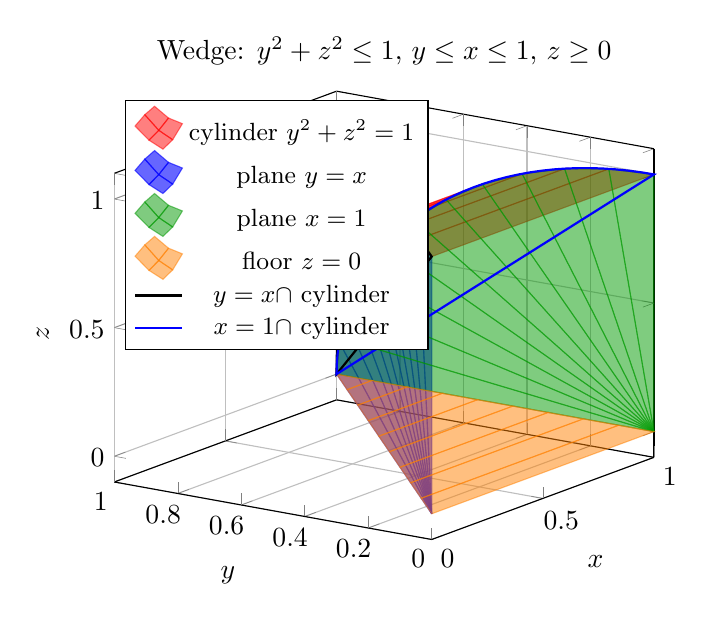
\begin{tikzpicture}
\begin{axis}[
    view={-55}{18},
    xlabel={$x$}, ylabel={$y$}, zlabel={$z$},
    grid=major,
    title={Wedge: $y^2+z^2\le 1$, $y\le x\le 1$, $z\ge 0$},
    legend style={font=\small, at={(0.02,0.98)}, anchor=north west},
    clip=false,
]
% Cylinder y^2+z^2=1, x from y to 1 (red)
\addplot3[surf, shader=flat, opacity=0.5, color=red,
    variable=\t, variable y=\s, domain=0:90, y domain=0:1,
    samples=12, samples y=2]
    ({cos(\t) + \s*(1-cos(\t))}, {cos(\t)}, {sin(\t)});
\addlegendentry{cylinder $y^2+z^2=1$}
% Plane y = x face (blue quarter disk in that plane)
\addplot3[surf, shader=flat, opacity=0.6, color=blue,
    variable=\t, variable y=\r, domain=0:90, y domain=0:1,
    samples=12, samples y=2]
    ({\r*cos(\t)}, {\r*cos(\t)}, {\r*sin(\t)});
\addlegendentry{plane $y=x$}
% Back face x = 1 (green quarter disk)
\addplot3[surf, shader=flat, opacity=0.5, color=green!60!black,
    variable=\t, variable y=\r, domain=0:90, y domain=0:1,
    samples=12, samples y=2]
    (1, {\r*cos(\t)}, {\r*sin(\t)});
\addlegendentry{plane $x=1$}
% Floor triangle z=0, 0<=y<=x<=1 (orange)
\addplot3[surf, shader=flat, opacity=0.5, color=orange,
    variable=\s, variable y=\u, domain=0:1, y domain=0:1,
    samples=10, samples y=2]
    ({\s + \u*(1-\s)}, {\s}, {0});
\addlegendentry{floor $z=0$}
% Edge curves
\addplot3[black, thick, domain=0:90, samples=40, variable=\t]
    ({cos(\t)}, {cos(\t)}, {sin(\t)});
\addlegendentry{$y=x\cap$ cylinder}
\addplot3[blue, thick, domain=0:90, samples=40, variable=\t]
    (1, {cos(\t)}, {sin(\t)});
\addlegendentry{$x=1\cap$ cylinder}
\end{axis}
\end{tikzpicture}
\end{document}